\documentclass[10pt,xcolor=pdflatex]{beamer}
\usepackage{newcent}
\usepackage[utf8]{inputenc}
\usepackage[slovak]{babel}
\usepackage{hyperref}
\usepackage{fancyvrb}
\usetheme{FIT}

%%%%%%%%%%%%%%%%%%%%%%%%%%%%%%%%%%%%%%%%%%%%%%%%%%%%%%%%%%%%%%%%%%
\title[FYO projekt]{Aberácie šošoviek}

\author[]{Roman Dobiáš}

\institute[]{Brno University of Technology, Faculty of Information Technology\\
Bo\v{z}et\v{e}chova 1/2. 612 66 Brno - Kr\'alovo Pole\\
xdobia11@stud.fit.vutbr.cz}

\date{April 16, 2019}
%\date{\today}
%\date{} % bez data

%%%%%%%%%%%%%%%%%%%%%%%%%%%%%%%%%%%%%%%%%%%%%%%%%%%%%%%%%%%%%%%%%%

\begin{document}

\frame[plain]{\titlepage}

\begin{frame}\frametitle{Aberácie šošoviek}
    \begin{itemize}
        \item def. \textit{odchíľka od idealizovaného modelu Gaussovej optiky} - Hecht
        \item def. \textit{neschopnosť optického systému zaostriť ľúče do jedného bodu} - Wikipedia
        \item skumané a definované \textbf{Ludwigom von Seidelom} (1821-1896)
        \item optika prvého rádu - \textbf{paraxiálna optika} - $n_1 \times \alpha_1 = n_2 \times \alpha_2$
    \end{itemize}
    \begin{figure}
        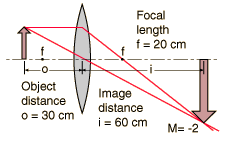
\includegraphics[scale=0.5]{img/thinLensEq.png}
        \caption{Model ideálnej tenkej šošovky}
    \end{figure}

\end{frame}

\begin{frame}\frametitle{Rozdelenie aberácii}
    \begin{itemize}
        \item \textbf{monochromatické} \\
            \begin{itemize}
                \item rozostrenie\\
                    \thinspace Spherical aberration, Coma, Astigmatism
                \item deformácia \\
                    \thinspace Petzval field curvature
            \end{itemize}
        \item \textbf{chromatické} \\
            \thinspace Chromatická aberácia
    \end{itemize}
    
\end{frame}


\begin{frame}\frametitle{Sférická aberácia}
    \begin{itemize}
        \item pararelné ľúče nie sú fokusované do jediného bodu\textit{optickej osi}
        \item \textbf{Dôsledok:} rozostretý obraz, \textit{circle of the least confusion}
        \item Riešienie: \textit{asférický tvar šošoviek}, korektory
    \end{itemize}

    \begin{columns}
    \column{0.5\textwidth}
    \begin{figure}
        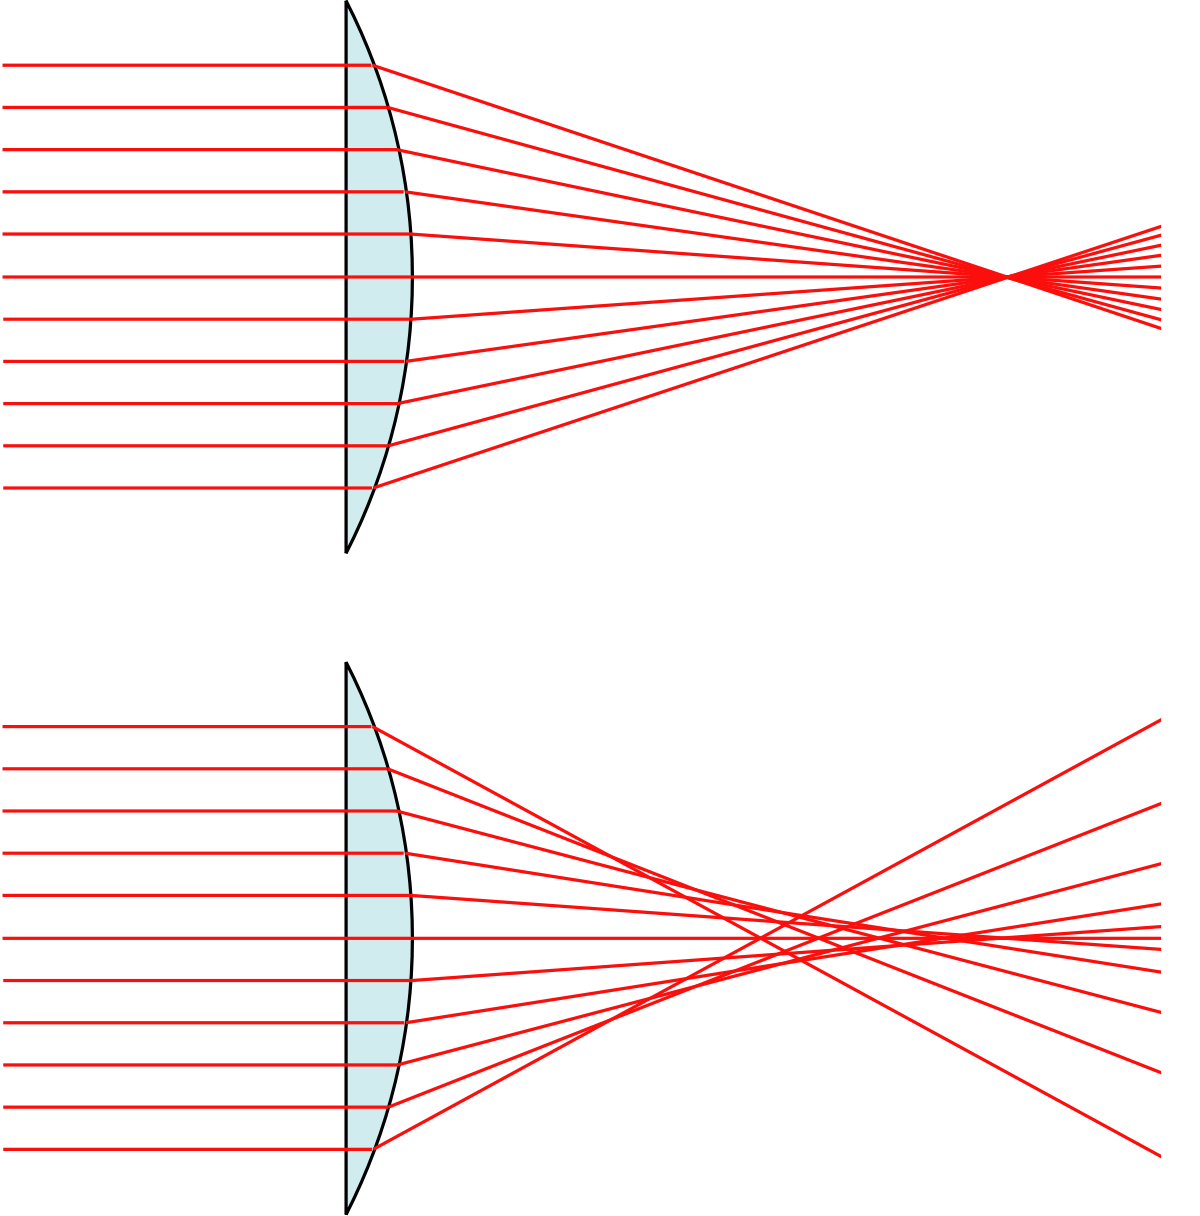
\includegraphics[scale=0.1]{img/sphericalAberrationWikipedia.png}
        \caption{Ideálna (hore) vs reálna šošovka (dole)}
    \end{figure}
    \column{0.5\textwidth}
    \begin{figure}
        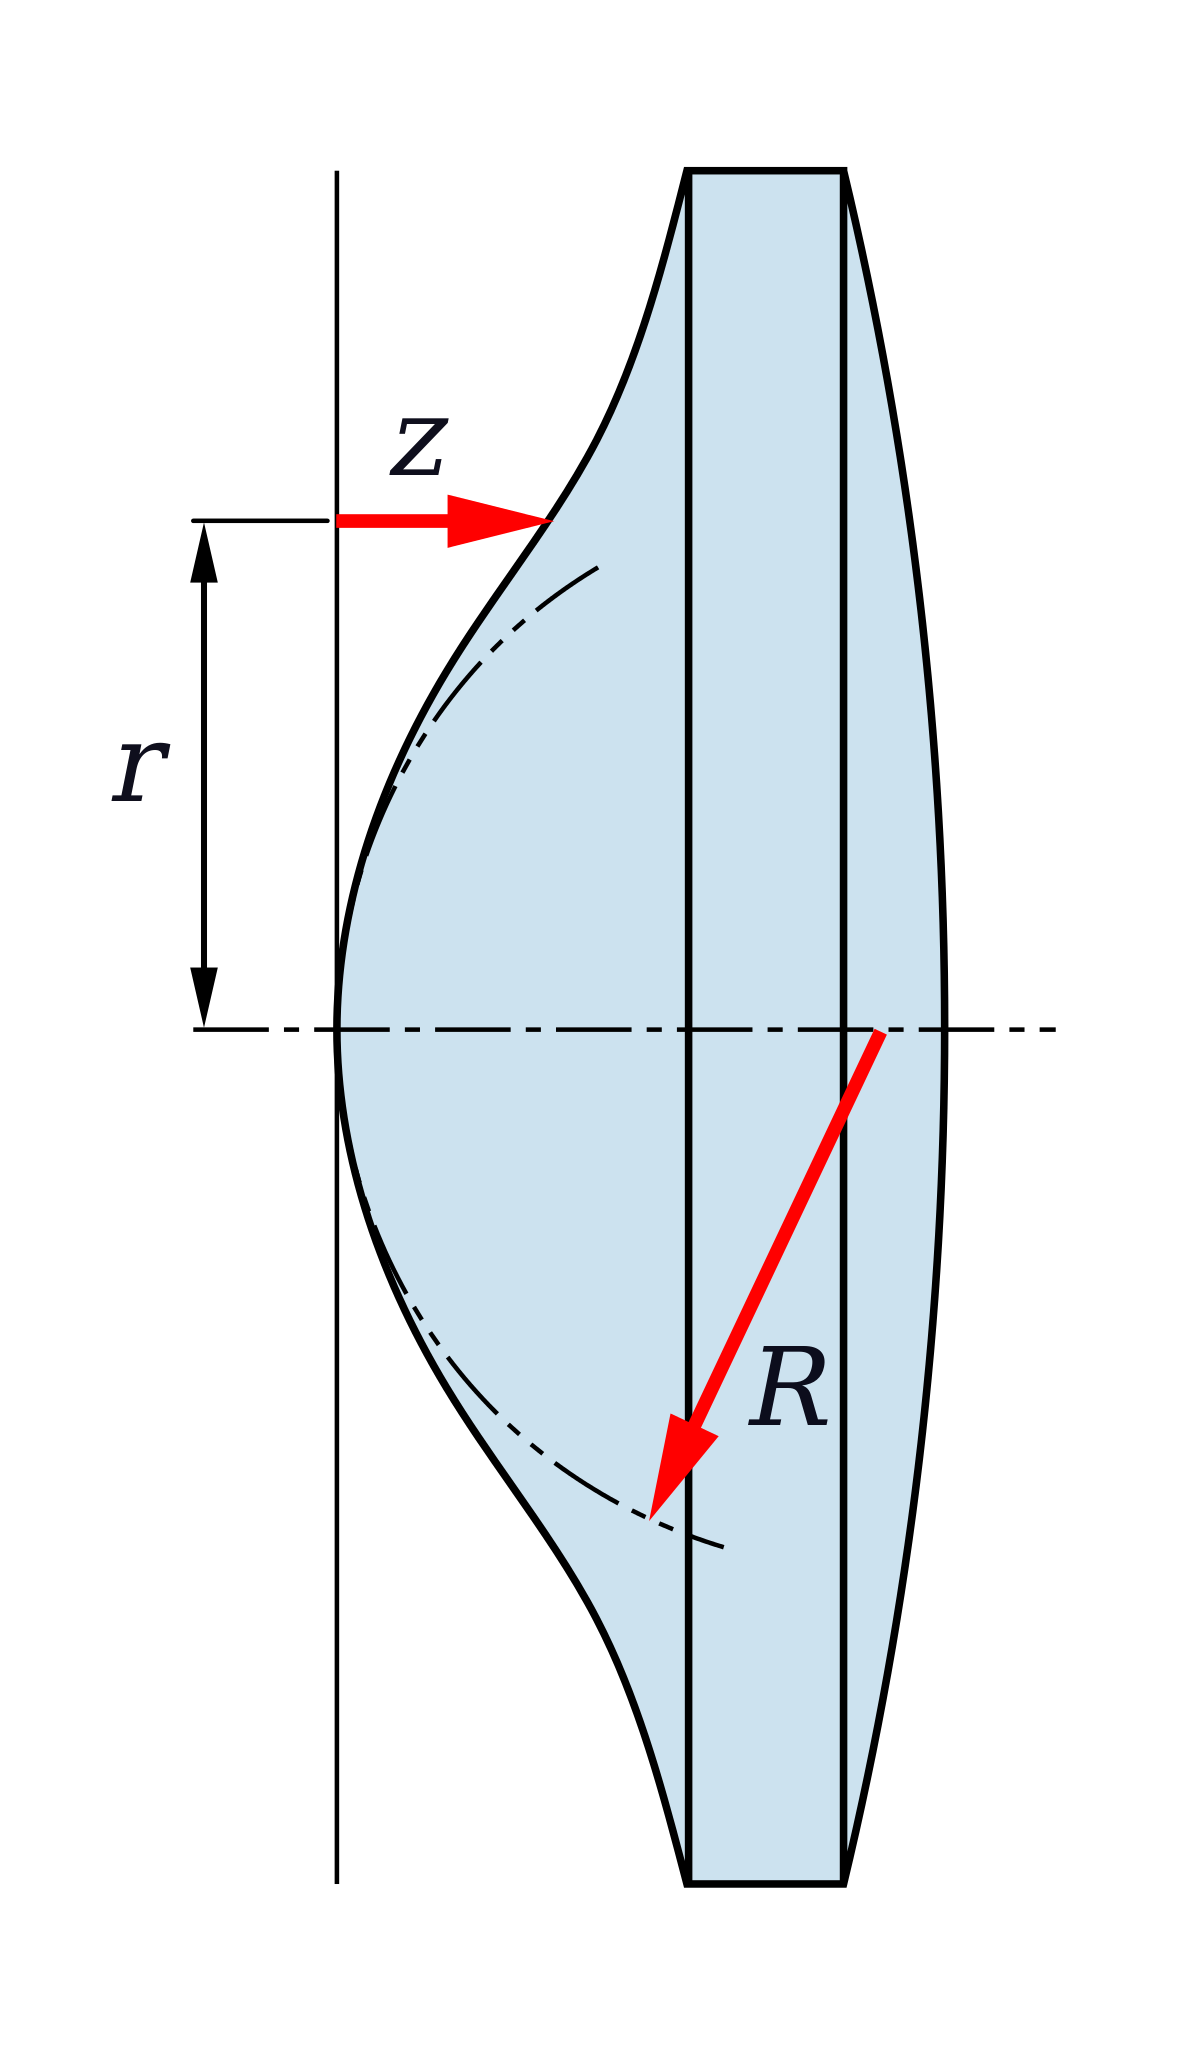
\includegraphics[scale=0.05]{img/asphericLen.png}
        \caption{Asférická šošovka}
    \end{figure}
    \end{columns}
\end{frame}


\begin{frame}\frametitle{Sférická aberácia}
    \begin{itemize}
        \item Hubblov teleskop 1990 (1.6 miliardy \$), opravný modul COSAR 
        \item Arecibo, Puerto Rico, najväčší radiotelskop na zemi, vysiaci korektor 
    \end{itemize}

    \begin{columns}
    \column{0.5\textwidth}
    \begin{figure}
        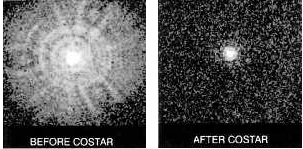
\includegraphics[scale=0.5]{img/cosar.png}
        \caption{Obraz z Hubblovho teleskopu pred a po korekcii}
    \end{figure}
    \column{0.5\textwidth}
    \begin{figure}
        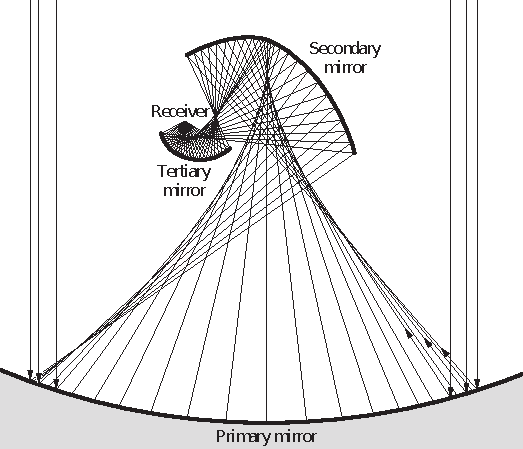
\includegraphics[scale=0.5]{img/arecibo.pdf}
        \caption{Arecibo, Puerto Rico}
    \end{figure}
    \end{columns}
\end{frame}



\begin{frame}\frametitle{Coma}
    \begin{itemize}
        \item rozmazanie bodových predmetov ležiacich mimo optickú osu 
        \item typickým prejavom je vznik chvosta (ang. \textit{coma}, česky \textit{ocas})
        \item \textbf{riešenie:} coma corrector, pre 1 vlnovú dĺžku aplanatické (asférické šošovky)
    \end{itemize}

    \begin{columns}
        \column{0.5\textwidth}
        \begin{figure}
            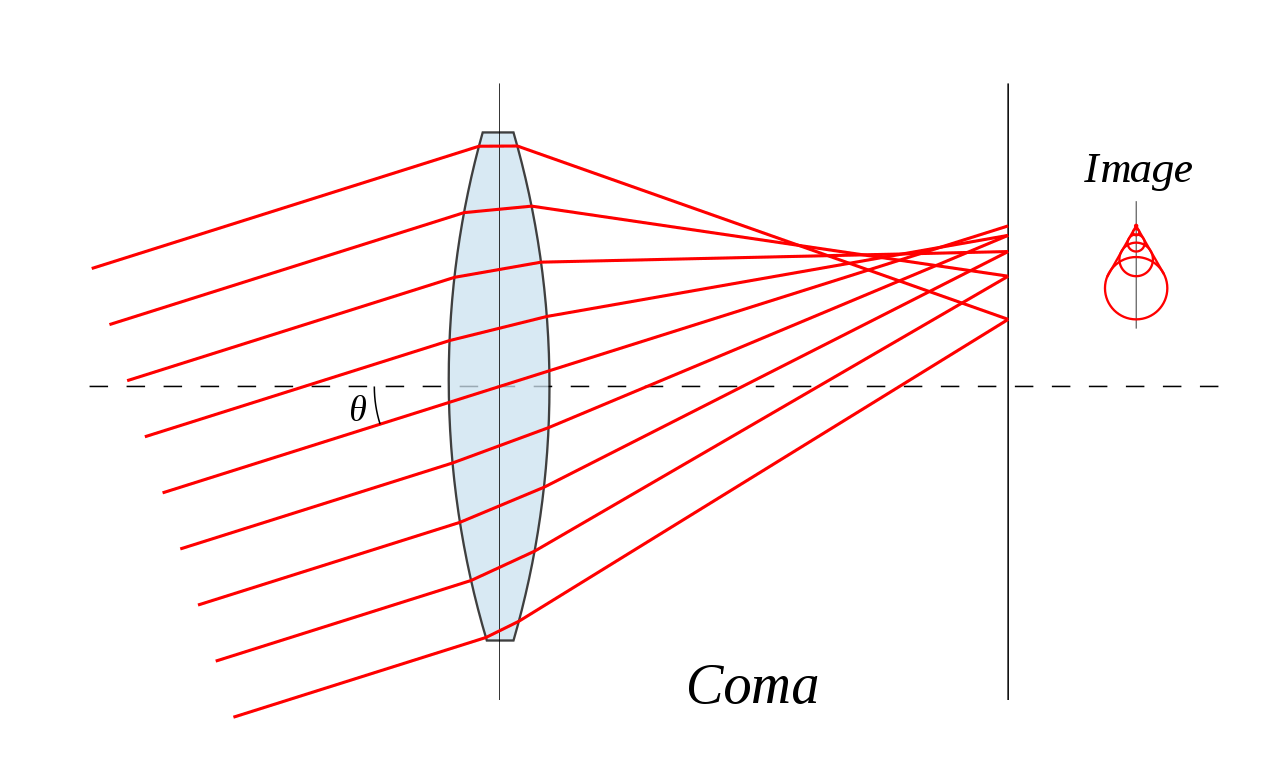
\includegraphics[scale=0.15]{img/coma.png}
        \end{figure}

        \column{0.5\textwidth}
        \begin{figure}
            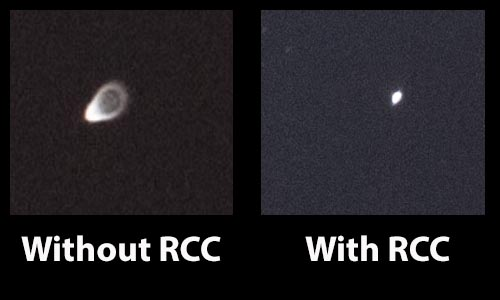
\includegraphics[scale=0.20]{img/coma.jpg}
            \caption{Baader Rowe Coma Corrector}
        \end{figure}
    \end{columns}
\end{frame}


\begin{frame}\frametitle{Petzvalovo zakrivenie pola}
    \begin{itemize}
        % http://www.wikiwand.com/en/Petzval_field_curvature
        \item lúče z naklonenej predmetovej roviny konvergujú na rovine 
        \item nemožno voliť obrazovú rovinu, nutno použiť zakrivenú rovinu
    \end{itemize}

    \begin{columns}
        \column{0.5\textwidth}
        \begin{figure}
            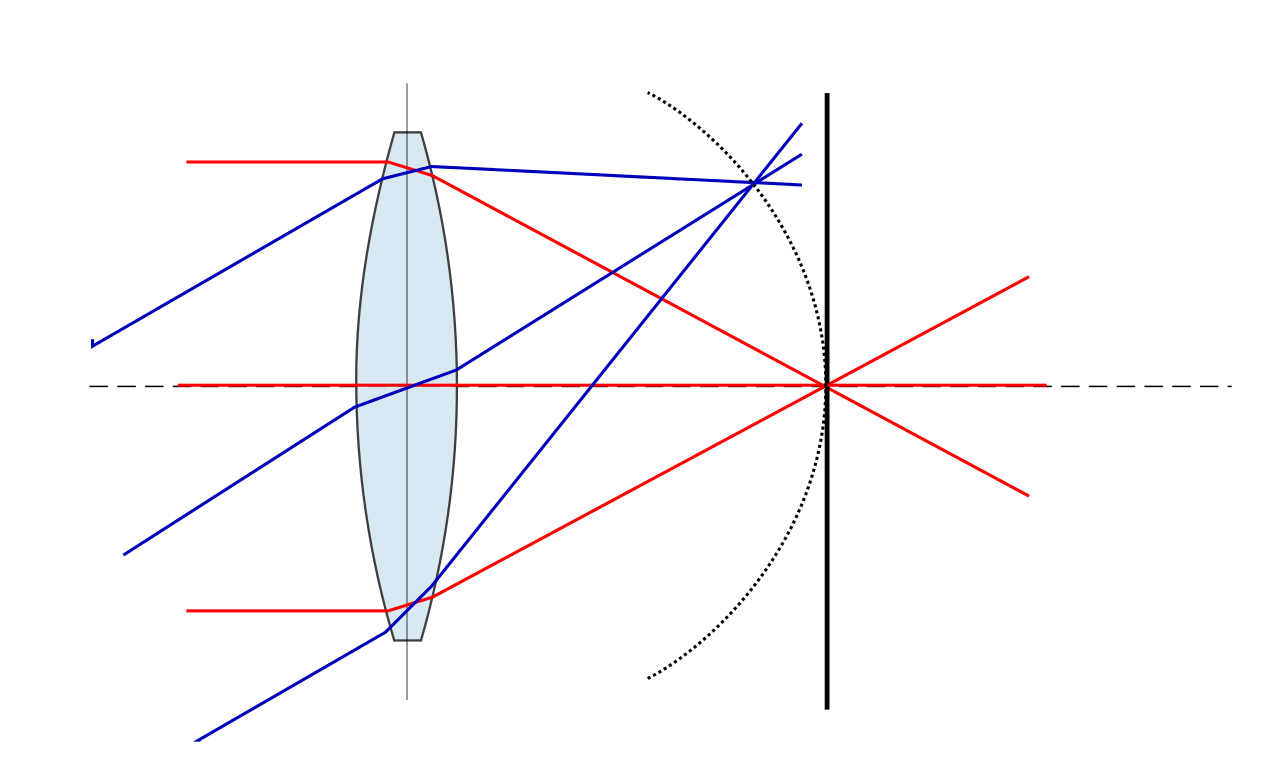
\includegraphics[scale=0.15]{img/fieldcurvature.png}
        \end{figure}
            \column{0.5\textwidth}
        \begin{figure}
            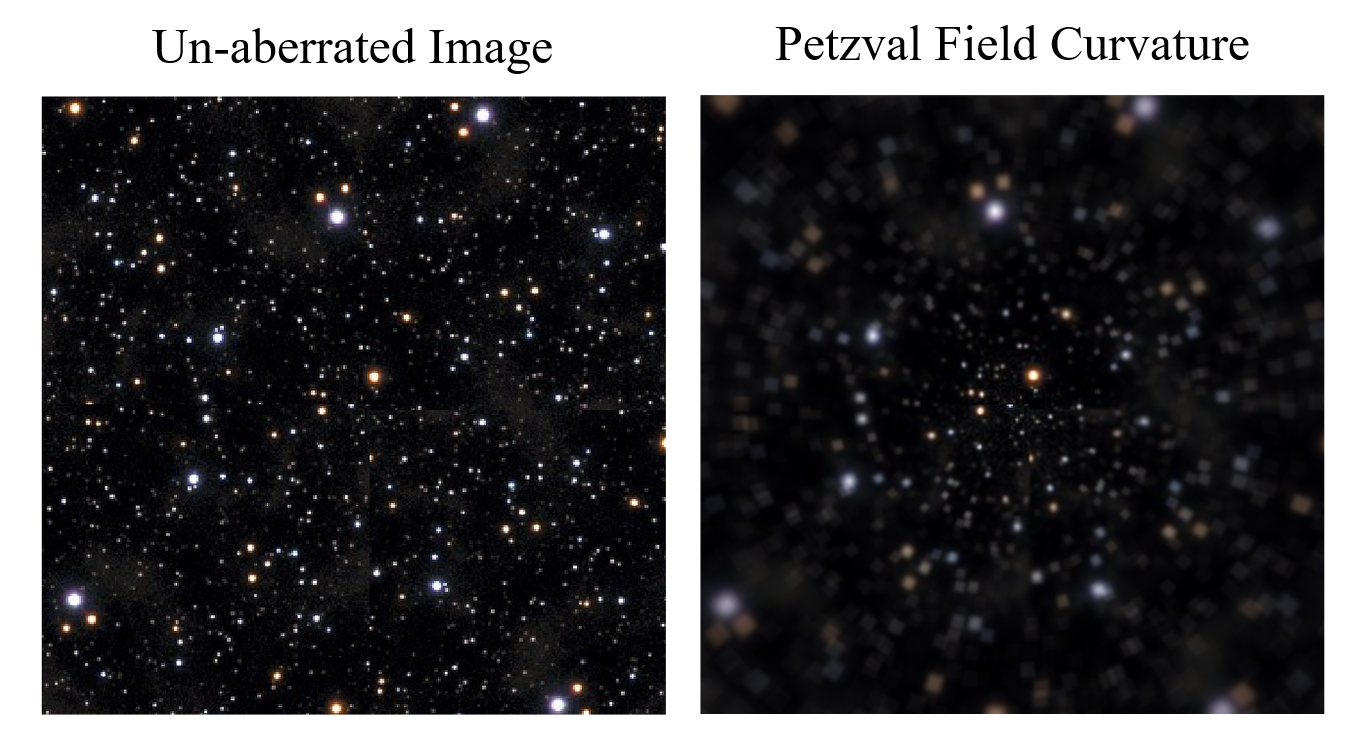
\includegraphics[scale=0.50]{img/fieldAberration.png}
        \end{figure}
    \end{columns}
\end{frame}
\begin{frame}\frametitle{Petzvalovo zakrivenie pola}
        \begin{figure}
            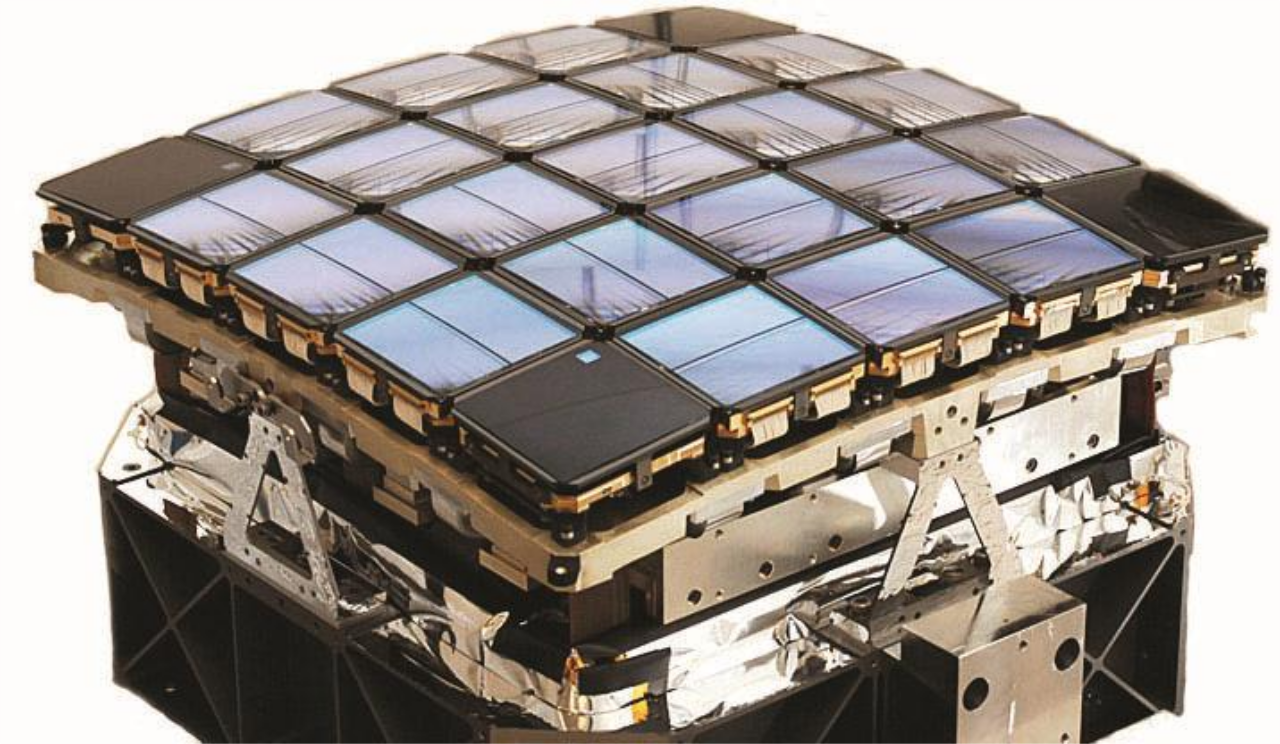
\includegraphics[scale=0.15]{img/kepler.png}
            \caption{Senzor v Kepler space observatory}
        \end{figure}
\end{frame}

\begin{frame}\frametitle{Astigmatizmus}
    \begin{itemize}
        \item lúče jednej roviny majú odlišné ohnisko od ľúčov roviny kolmej na ňu
    \end{itemize}
    \begin{figure}
        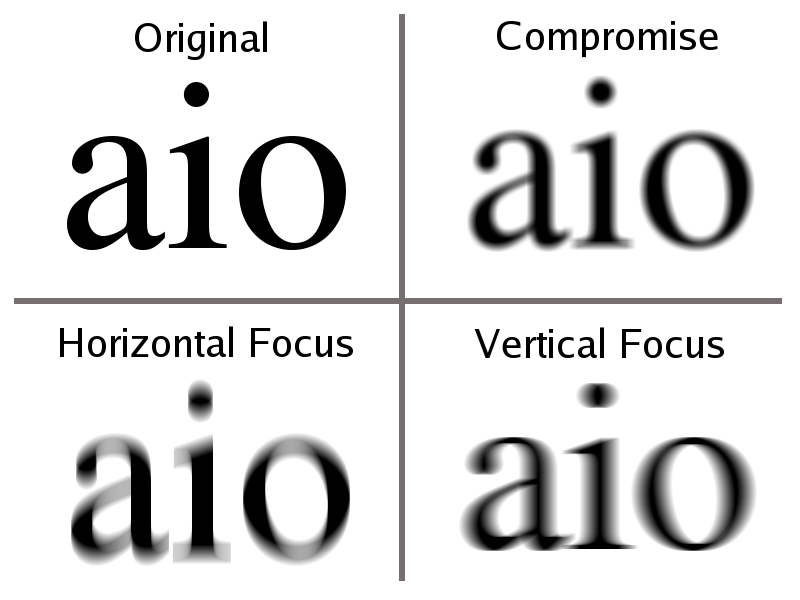
\includegraphics[scale=0.20]{img/astigmatism.png}
        \caption{Vizuálny astigmatizmus}
    \end{figure}
\end{frame}

\begin{frame}\frametitle{Chromaticka aberácia}
    \begin{itemize}
        \item index lomu je funkciou \textbf{vlnovej dĺžky}
        \item \textbf{Dôsledok:} rozostrenie podľa farebných zložiek
        Riešienie: \textit{doublet}, SW korekcia 
    \end{itemize}

    \begin{columns}
        \column{0.4\textwidth}
    \begin{figure}
        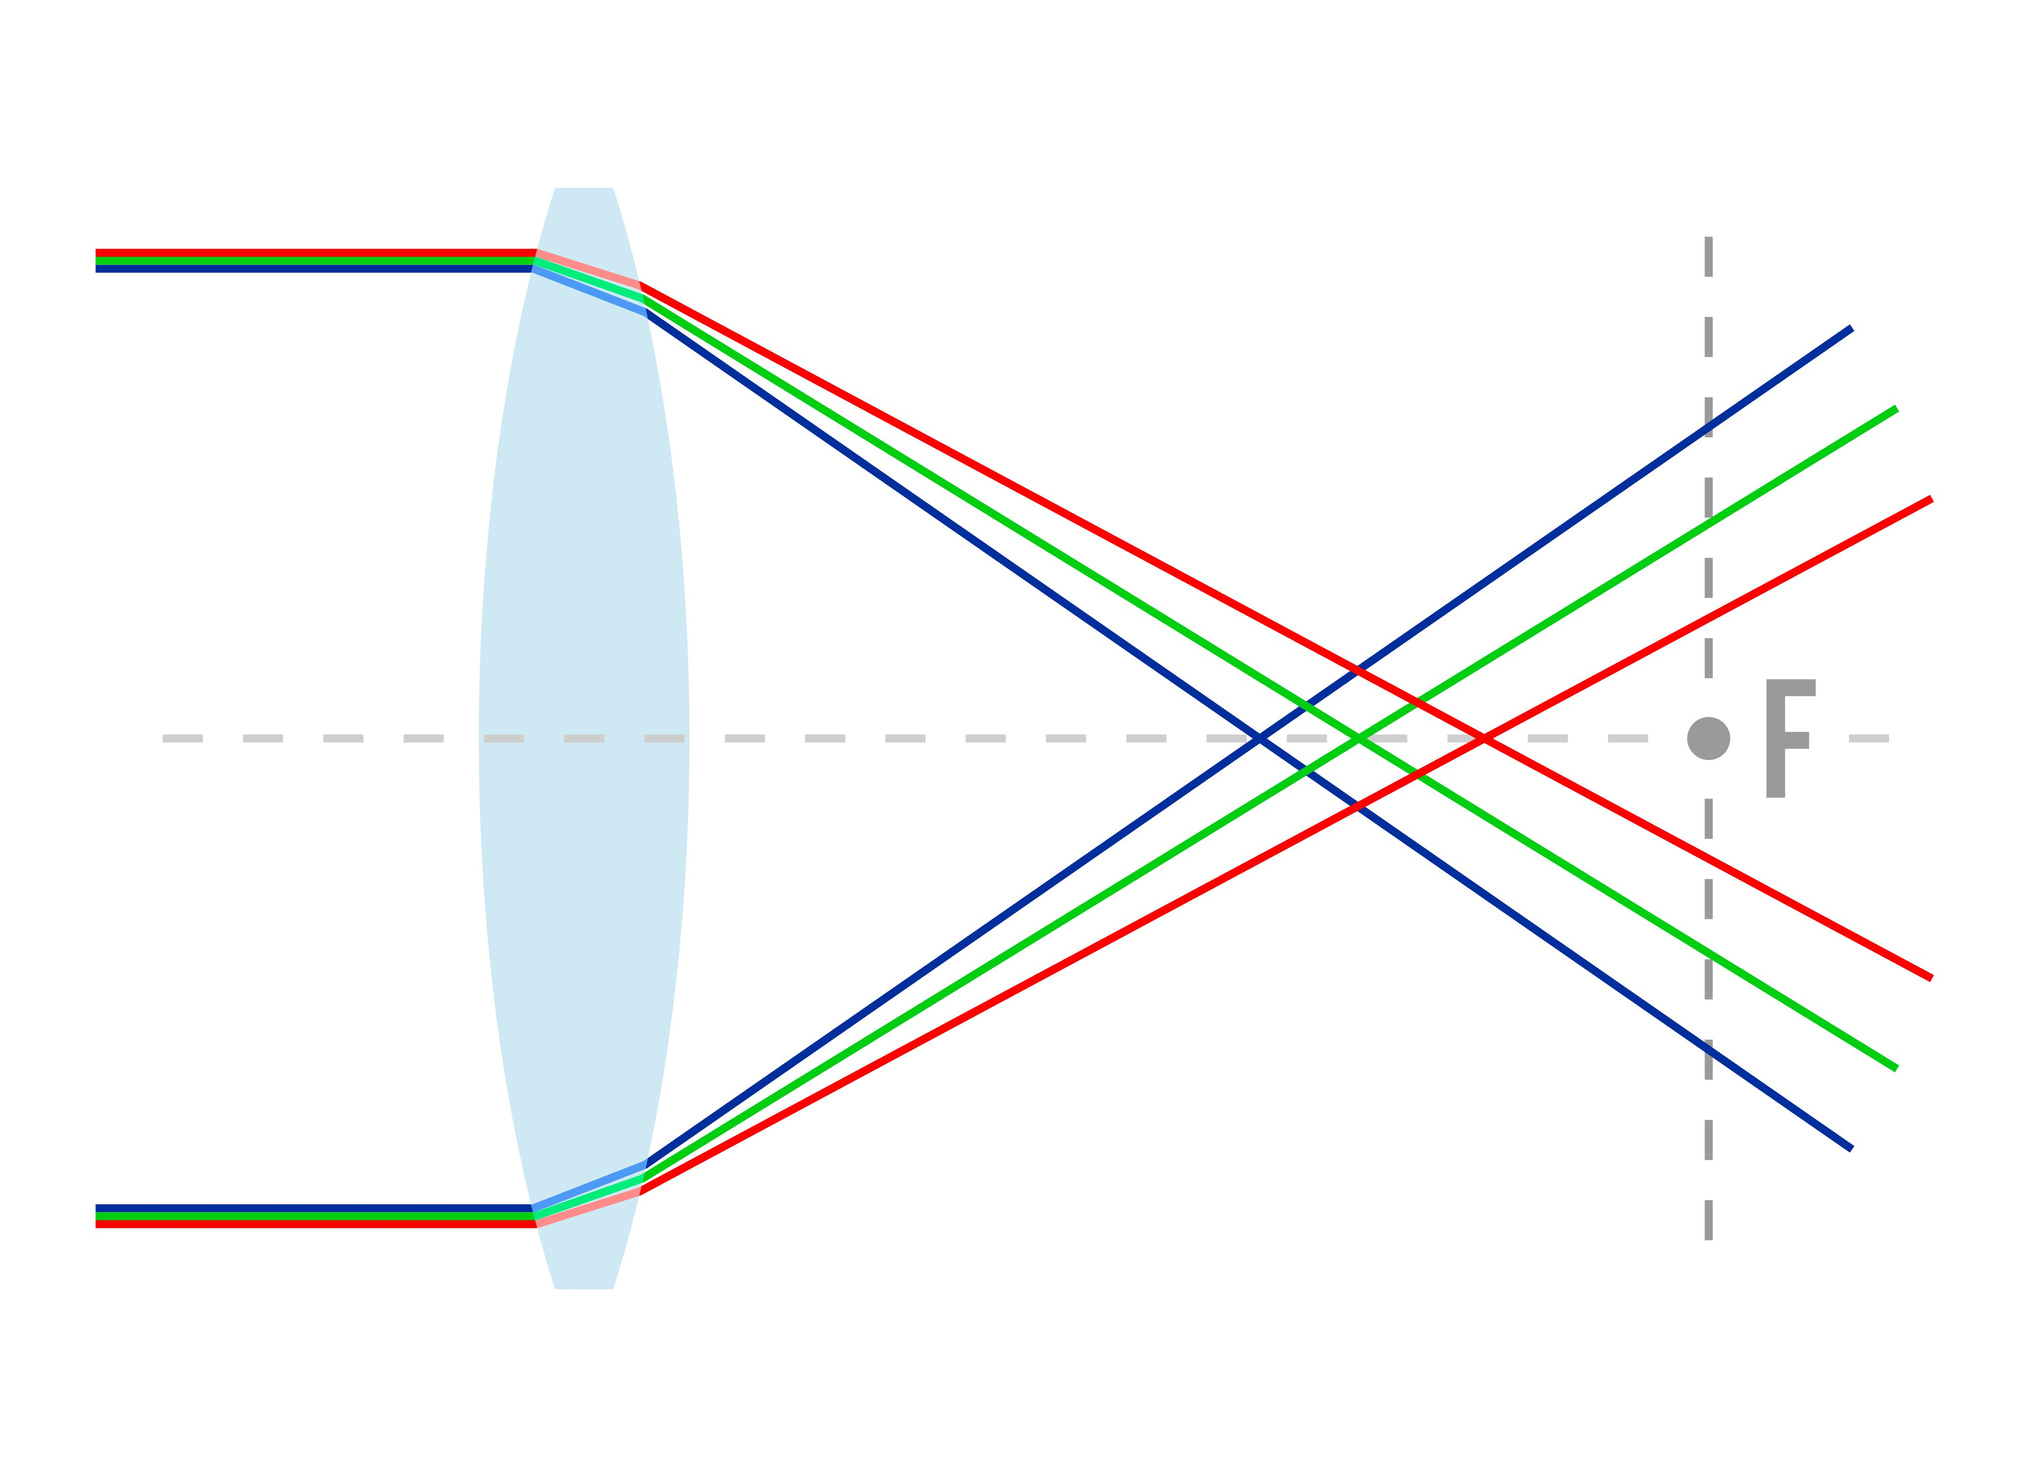
\includegraphics[scale=0.3]{img/chromaticFocus.jpg}
        \caption{Disperzia na šošovke}
    \end{figure}

        \column{0.6\textwidth}
    \begin{figure}
        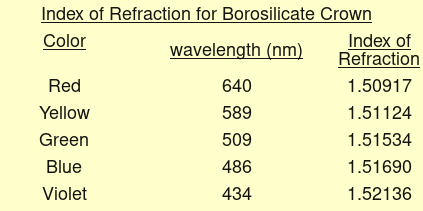
\includegraphics[scale=0.4]{img/chromaticRefraction.png}
        \caption{Závislosť indexu lomu na vlnovej frekvencii}
    \end{figure}
    \end{columns}
\end{frame}

\begin{frame}
    \begin{figure}
        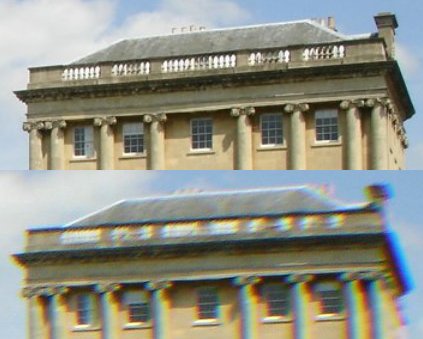
\includegraphics[scale=0.4]{img/chromaticAberrationWikipedia.jpg}
        \caption{Dôsledok chromatickej aberácie vo výslednom obraze}
    \end{figure}
\end{frame}

\begin{frame}\frametitle{Projekt}
    \begin{itemize}
        \item 2D raytracer
        \item HTML, Javascript, canvas, Pixi.js
    \end{itemize}

    \begin{figure}
        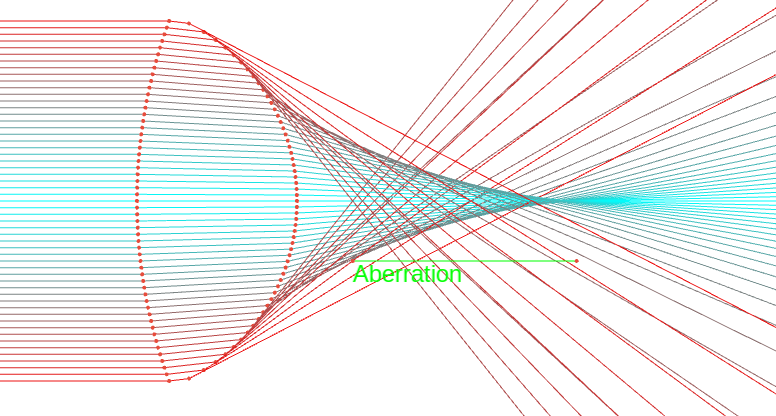
\includegraphics[scale=0.35]{img/application.png}
    \end{figure}
\end{frame}

%\bluepage{
%        Ďakujem za vašu pozornosť 
%        Everything will be okay in the end. If it's not okay, then it's not the end
%    John Lenon
%}
\frame[plain]{%
\begin{beamercolorbox}[left,colsep=0pt,rounded=false,wd=\paperwidth,ht=\paperheight]{title}
\usebeamerfont{title}
\vbox to \paperheight {\vfill 
    \hbox to \paperwidth {
        \hfill Ďakujem za vašu pozornosť \hfill
    }
    \vspace{1cm}
    \hbox to \paperwidth {
      \hfill \small ``Everything will be okay in the end. If it's not okay, \hfill
    }
    \hbox to \paperwidth {
        \hfill \small then it's not the end.'' - \textbf{John Lenon} \hfill
    }
    \vspace{1cm}
    \hbox to \paperwidth {
        \hfill \scriptsize Zdroje:\hfill
    }
    \hbox to \paperwidth {
        \hfill \scriptsize Hecht,Optics, Pearson education, Addison-Wesley, 2002\hfill
    }

    \hbox to \paperwidth {
        \hfill \scriptsize Wikipedia.com\hfill
    }

  
    
    \vfill }
\end{beamercolorbox}%
}
\end{document}
